\section{Benchmark mémoire}\label{sec:dmlmem}


\textbf{TODO BIG en GB etc.........}
\textbf{TODO image en plus grandes}

    La section suivante présente notre benchmark mémoire appelé \textit{Demonstrate Memory Limit} ou \verb=DML_MEM=. Cet outil permet de vérifier le bon comportement de la hiérarchie mémoire lors d'accès mémoire à un jeu de donnée par sauts de taille constante. 

    

    \subsection{Motivations}
    %%%%%%%%%%%%%%%%%%%%%%%%%%%%%%%%%%%%%%%%%%%%%%%%%%%%%%
    
        L'industrie de la recherche pétrolière est un grand consommateur de calcul haute performance. Les applications utilisées utilisent des algorithmes de \textit{stencil}\footnote{En mathématiques, en particulier dans le domaine de l'analyse numérique, un stencil est un arrangement géométrique d'un réseau nodal qui se lie au point d'intérêt en utilisant une routine d'approximation numérique. Les stencils sont à la base de nombreux algorithmes de résolution numérique des équations aux dérivées partielles (wikipédia).} qui impliquent des accès mémoire réguliers non contigus par \textit{sauts} aussi appelés \glspl{stride}. D'autres applications comme le calcul matriciel parcourent des matrices et génèrent des accès mémoire par saut de taille constante (multiple d'une taille d'une ligne). La \autoref{pic:dml_strides_acces_main} expose un exemple simple de tels accès. D'autres algorithmes peuvent réaliser ce genre d'accès par \textit{strides} comme les multiplications de matrices, les transformées de Fourrier ou le parcours d'un tableau de structures pour accéder à certains champs. Si les objets sont stockés continûment en mémoire, l'accès à un même champ de chaque objet réalise en réalité des accès mémoire par saut de taille fixe. 
        
        
        \textbf{TODO reprendre c'est trop petit}
        \begin{figure}[ht]
            \centering
                \begin{subfigure}[b]{0.25\linewidth}
                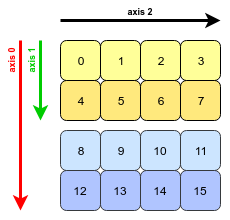
\includegraphics[width=\linewidth]{images/dml_strides_acces_matrix.png}
                \caption{Accès en ligne ou en colonne à une matrice.}
                \label{pic:dml_strides_acces_matrix}
                \end{subfigure}
            ~ %add desired spacing between images, e. g. ~, \quad, \qquad, \hfill etc. 
            %(or a blank line to force the subfigure onto a new line)
                \begin{subfigure}[b]{0.60\linewidth}
                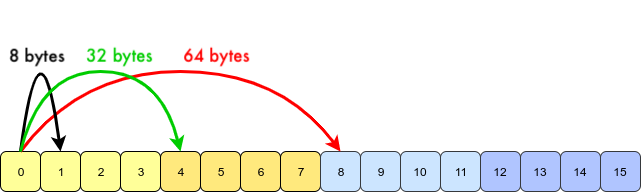
\includegraphics[width=\linewidth]{images/dml_strides_acces.png}
                \caption{Les accès en ligne ou en colonne impliquent des sauts en mémoire de tailles différentes.}
                \label{pic:dml_strides_acces}
                \end{subfigure}
            \caption{Exemple d'une application réalisant des accès en colonne à une matrice. Ces accès impliquent en réalité des sauts entre les adresses mémoires utilisées.}\label{pic:dml_strides_acces_main}
        \end{figure}
        % \subsubsection{Motivations}
    
    
        La grande majorité de ces applications ne réalisent pas suffisamment de calcul sur une donnée transférée pour masquer le temps de son accès mémoire. Ce déséquilibre de performance de l'architecture limite la performance de ces codes par celle du bus mémoire. 
        Pour ces applications, il est primordial que l'architecture soit capable d'anticiper le maximum d'accès mémoire grâce à son matériel de prélecture mémoire (\textit{memory prefetcher} \textbf{todo GLS avec le suivant -->}). Les \glspl{prelecteur} mémoires sont conçus pour anticiper les accès avant qu'ils ne soient réalisés pour réduire la latence d'accès. Lorsque les accès sont simples (taille régulière, proches en mémoire), la majorité des architectures modernes obtiennent de très bonnes performances. Cependant, les accès par sauts peuvent être grands (supérieurs à plusieurs lignes de cache) et lorsque de multiples accès sont réalisés en concurrence, le prélecteur peut rencontrer des difficultés à les anticiper. De plus, si le prélecteur mémoire anticipe de mauvais accès, le bus mémoire sera saturé de données inutiles au calcul. Le bus mémoire étant la ressource critique pour la majorité des applications HPC, il est primordial que son utilisation soit la plus efficace possible.  
    
        

    \subsubsection{Objectifs}
        
        Le développement du benchmark \verb=DML_MEM= a été réalisé pour répondre à trois objectifs:
        \begin{enumerate}
            \item \textbf{Caractériser la performance} d'une architecture pour l'exécution d'applications utilisant un motif d'accès mémoire par strides. En mesurant ses performances, il est ensuite possible de prouver l’efficacité de l’utilisation du sous-système mémoire pour une application réelle utilisant ce type d'accès. En effet, nous montrons que pour vérifier la bonne performance d'une architecture pour une application donnée, il n'est pas suffisant de vérifier que le bus mémoire est saturé.
            \item \textbf{Attirer l'attention du programmeur} sur la complexité des architectures et de son impact sur les performances d'un code. Le benchmark développé doit pouvoir être utilisé pour caractériser l'ensemble de la hiérarchie mémoire: fonctionnement des caches et du prélecteur mémoire, saturation du bus mémoire, impact de l'utilisation de plusieurs coeurs... En appréhendant cette complexité, il sera plus simple pour le programmeur d'apporter les bonnes modifications à son code pour tirer la pleine performance du bus mémoire.
            \item \textbf{Aider à la conception} de nouvelles architectures en utilisant le benchmark pour vérifier le bon fonctionnement du système mémoire. En effet, en utilisant ce benchmark, nous avons trouvé plusieurs dysfonctionnements majeurs dans un accélérateur prévu pour ce type d'applications \textbf{TODO cest quoi CE TYPE}. Grâce à notre outil, nous avons pu prouver que les performances théoriques de la plateforme n'étaient pas accessibles par l'application. 
        \end{enumerate}

    
    \subsubsection{Comparaison avec l'existant}
    %%%%%%%%%%%%%%%%
        L'étude des différents benchmarks existants est réalisée dans la \autoref{sec:edl_perf_intro}.  Au moment de la réalisation de ce travail de thèse, il n’existe à notre connaissance aucun benchmark permettant de caractériser l’architecture pour ce type d’accès. Le benchmark s’approchant le plus de cet objectif est celui de Saavedra \cite{Saavedra1995}. Il utilise une taille de saut fixée au début de l’exécution pour accéder à un jeu de données. Cependant, la taille de ce dernier doit être un multiple d’une puissance de 2 et ne permet pas de dépasser la taille du dernier niveau de cache. Comme le souligne \cite{Yotov2005}, le problème d’une telle approche est de vouloir mesurer tous les niveaux de la hiérarchie simultanément. Les mesures peuvent alors être influencées par certains paramètres des différents niveaux de caches. Ces mesures doivent être interprétées par l’utilisateur, le programme ne créant pas automatiquement la hiérarchie. Un second outil s'approchant de notre démarche est le benchmark \verb|DISBench| \cite{disbench}. Cependant, il ne bénéficie d'aucune méthode solide de vérification de la performance comme celle implémentée par \verb=DML_MEM=. De plus, il n'est, en aucun cas, prévu pour faciliter le test de multiples tailles de strides sur différentes tailles de jeux de données. Le code n'est plus maintenu depuis 6 ans et ne peut pas être exécuté sans erreur lors de l'exécution.


\subsection{Le benchmark DML\_MEM}
%%%%%%%%%%%%%%%%%%%%%%%%%%%%%%%%%%%%%%%%%%%%%%%%%%%%%%
    Le motif d'accès par \gls{stride} est donc très courant dans le calcul haute performance. La distance entre deux accès peut varier d'une application, ou d'un jeu de données, à l'autre. Pour caractériser les plateformes pour ces applications, il est donc nécessaire de posséder un benchmark paramétrable permettant de faire varier la taille du jeu de données et la taille du saut. Cette section présente comment le benchmark \verb=DML_MEM= a été développé. Grâce à de nombreuses options nous montrons comment différentes parties de la microarchitecture peuvent être testée: caches, TLB, bus mémoire.


    \subsubsection{Concept}
    %%%%%%%%%%%%%%%%
        
        Le principe du benchmark est d'accéder à un tableau en utilisant différentes tailles de strides. Pour chaque stride une mesure de performance est réalisée. Une fois toutes les tailles de stride mesurée, le benchmark augmente la taille du jeu de données utilisé (voir \autoref{pic:dml_stride_intro}). La vitesse d'évolution de la taille des strides et du jeu de données peut être paramétrée. Les accès peuvent être réalisés en lecture ou en lecture/écriture.
       
        \begin{figure}[ht]
        \center
        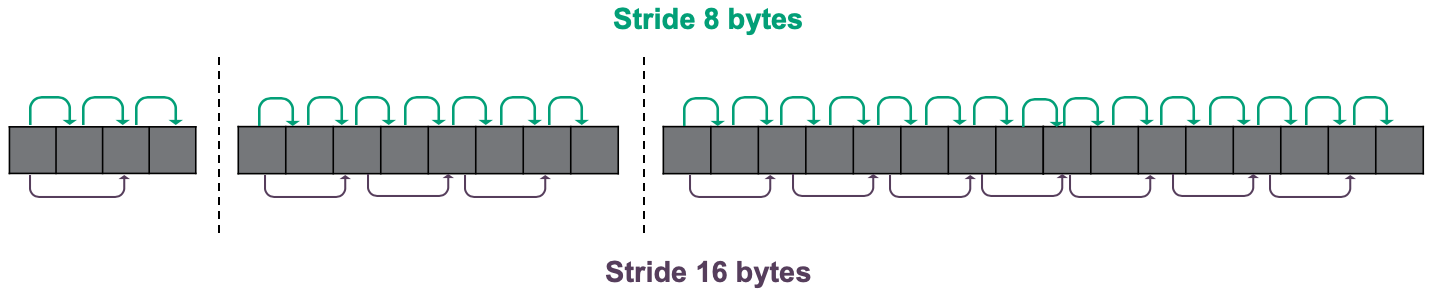
\includegraphics[width=14cm]{images/dml_stride_intro.png}
        \caption{\label{pic:dml_stride_intro}Évaluation de la performance de deux tailles de stride (8 et 16 bytes) sur trois jeux de données de tailles différentes.}
        \end{figure}
        \textbf{todo plus gros le texte ?}


        Le benchmark se déroule en deux étapes: la configuration et son exécution.
        Lors de la configuration, les différents paramètres nécessaires pour l'exécution du benchmark sont extraits de la ligne de commande ou utilisent, le cas échéant, des valeurs par défaut. Les différentes versions du benchmark (mode d'accès, taille du déroulement des boucles) sont toutes compilées, l'initialisation utilise un pointeur de fonction vers la bonne version requise par l'utilisateur. Ensuite, le jeu de données est initialisé (voir \autoref{sec:dml_init}). 
        La deuxième étape consiste à exécuter le benchmark et à mesurer ses performances. Pour une taille de jeu de donnée et une taille de stride, la bande passante effective maximale, minimale ou moyenne est mesurée et affichée. Pour cela, le benchmark mesure le temps nécessaire pour réaliser le noyau de calcul. Celui-ci, renvoie le nombre d'accès réalisés grâce à l'initialisation du tableau durant la première étape. 
            \begin{verbatim}
time1 = get_micros();
num_ops = p->m_BENCHMARK();
time2 = get_micros();
bande_passante = calcul_bw(num_ops, time2 - time1);
            \end{verbatim}
            
        Ces mesures sont affichées au fur et à mesure de l'avancée du benchmark ainsi que dans un fichier de \textit{log}. Ce fichier peut ensuite être utilisé par un script pour afficher l'évolution de la performance de chaque stride en fonction de la taille du jeu de donnée. 
            
\begin{verbatim}
>./dml --type read --cacheline 64 --matrixsize 10000 --stride 8,64,256
...
Stride  S   ->          8         64        256
Value       ->    AVERAGE    AVERAGE    AVERAGE
       7.0 KiB     117.46          -          -
      81.0 KiB     114.29      88.24      74.12
      76.3 MiB      80.87      13.41       8.61
       7.5 GiB      80.35      13.11       7.18
...
\end{verbatim}

  

    \subsubsection{Les options}
    %%%%%%%%%%%%%%%%
        Le benchmark \verb=DML_MEM= accepte de nombreuses options. Grâce à celles-ci, différentes configurations peuvent être utilisées et permettent tester différents scénarios sur différentes parties de la microarchitecture. Nous décrivons ici les options les plus utiles pour l'utilisateur. Les nombreuses options peuvent être affichées avec l'option \verb|--help|.
        
        
        \paragraph{-{}-stride, -{}-minstride, -{}-maxstride, -{}-stridemode} Ces quatre premières options permettent de définir quelles sont les différentes strides à utiliser pour réaliser les mesures. La première d'entre elles, permet à l'utilisateur de choisir une ou plusieurs à réaliser. Pour cela, une liste de taille de strides séparées par des virgules doit être entrée. Les trois dernières options permettent de générer automatiquement des strides à utiliser dans un intervalle $[min, max]$. L'option \verb|--stridemode| peut être utilisée avec les valeurs \textit{even} et \textit{odd} pour décaler les strides ainsi générées. Cela permet d'éviter des strides utilisant seulement des multiples de deux, pouvant être affectées par certaines caractéristiques de la microarchitecture (taille de la ligne de cache, capacité des caches...). 
        
        \paragraph{-{}-matrixsize, -{}-minlog, -{}-maxlog, -{}-steplog, -{}-log} Ces 5 options permettent de définir la taille des jeux de données à utiliser. Leur taille évolue plus ou moins rapidement en fonction de la valeur de \verb|--steplog| jusqu'à atteindre la taille \verb|maxlog| ou bien celle de la matrice donnée avec l'option \verb|--matrixsize|. Si \verb|--steplog| est utilisé avec la valeur $0$, le benchmark réalise la mesure sur un seul jeu de données de la taille \verb=matrixsize=. L'option \verb|--log| permet de donner la même valeur à \verb|min| et \verb|max| pour ne réaliser la mesure que sur une taille de jeu de données. Couplée avec l'option \verb|--stride|, l'option \verb=--log= permet d'utiliser le benchmark pour n'accomplir qu'une seule mesure: un jeu de donnée, une stride.
        
        Ces 9 premières options sont les options principales du benchmark. Elles permettent de réaliser une multitude de mesures: performance des niveaux de caches, performance de la mémoire, fiabilité du \gls{prelecteur}, mesure de la taille d'une ligne de cache. Dans la \autoref{sec:dml_bad_stride} nous montrons comment ces options peuvent être utilisées pour identifier des tailles de strides ayant de mauvaises performances.
    
    
        \paragraph{-{}-type, -{}-unroll, -{}-mode} Ces trois options permettent de choisir le benchmark à utiliser. L'option \verb|--type| permet de réaliser les accès en lecture ou en lecture/écriture. La deuxième option permet d'appliquer l'optimisation du déroulement de boucle dont les différentes versions (déroulement de 2 à 64 fois) ont été programmées manuellement. La troisième option permet de choisir le mode d'accès. Par exemple, l'utilisation de différents pointeurs pour réaliser plusieurs accès notamment lorsque l'option \verb|--unroll| est utilisée. L'analyse de la performance de ces options est réalisée dans la \autoref{sec:dml_unroll}.

        \paragraph{-{}-hugepages} Cette option permet d'allouer la mémoire pour le jeu de données en utilisant des pages de 2 MiB contre 4 KiB habituellement. Un exemple de caractérisation des pages larges est présenté dans la \autoref{sec:dml_large_page}.
        
        \paragraph{-{}-annotate} Cette option est utilisée lorsque l'activité du bus mémoire est mesurée avec l'outil \verb=YAMB= présenté dans la \autoref{sec:yamb}. Le benchmark annote le graphique lorsqu'une nouvelle taille de stride ou de jeu de données est utilisée. Grâce à cette option, il est possible de corréler l'activité du bus avec une configuration particulière du benchmark. Cette option est utilisée dans la \autoref{sec:dml_cache_ok} pour mesurer l'activité du bus mémoire lorsqu'un jeu de donnée de la taille du dernier niveau de cache est utilisé. 

        \paragraph{Version parallèle} La dernière configuration du benchmark est la version parallèle utilisant MPI. Celle-ci doit être générée grâce à l'outil \textit{cmake} et la commande \verb|cmake -DOPT_BUILD_MPI=ON|. Grâce à cette version, plusieurs coeurs peuvent exécuter la même version du benchmark. Cette version du benchmark nous permet dans la \autoref{sec:dml_saturation} d'étudier l'évolution du débit mémoire lorsque des coeurs supplémentaires sont utilisés.
        
    
    \subsubsection{Validation des résultats} \label{sec:dml_init}
    %%%%%%%%%%%%%%%%

        Une grande difficulté lors de l'élaboration d'un benchmark a été de s'assurer que la performance mesurée était bien celle du code attendu. En effet, le compilateur peut appliquer certaines optimisations pour accélérer l'application. Ensuite, l'architecture elle-même peut se rendre compte de l'artificialité du code et en court-circuiter une partie. Dans les deux cas, le problème est que la mesure de la performance ne rend pas compte de la réalité du code et de la mesure attendue par le programmeur. 
        
        Pour éviter ces deux pièges, le benchmark \verb=DML_MEM= initialise le jeu de données avec deux valeurs suivant le type de l'accès voulu (lecture ou lecture/écriture). Lorsque le benchmark utilise des accès en lecture, le jeu de données est initialisé avec la valeur \textbf{1}, car chaque lecture occasionne un transfert sur le bus mémoire. 
        Lorsque le benchmark utilise le mode de lecture/écriture, le jeu de données est initialisé avec la valeur \textbf{2}. Chaque ligne doit être lue puis réécrite occasionnant deux passages sur le bus mémoire. Pour chaque accès, la valeur contenue dans le tableau est stockée dans une variable de compteur.  L'utilisation de chaque valeur pour l'ajouter au compteur empêche le compilateur et l'architecture d'appliquer certaines optimisations. À la fin de l'exécution, le benchmark retourne cette variable permettant de compter le nombre total d'accès \textbf{effectivement} réalisés.
        

    
    
    
    
    
    
    
    
\subsection{Expérimentations et principaux résultats}
%%%%%%%%%%%%%%%%%%%%%%%%%%%%%%%%%%%%%%%%%%%%%%%%%%%%%%

    Dans cette section nous présentons les principaux résultats obtenus avec le benchmark \verb=DML_MEM=. L'objectif est de montrer au lecteur les différentes mesures rendues possibles par l'utilisation de l'outil. Les tests sont principalement réalisés sur l'architecture des processeurs Intel Skylake. 


    \subsubsection{Impact du choix du compilateur sur la performance}
    %%%%%%%%%%%%%%%%
    
        Contrairement au benchmark du générateur de kernel (voir \autoref{sec:kg}), le code de \verb=DML_MEM= n'est pas écrit directement en assembleur. La qualité du compilateur peut donc avoir un impact significatif sur ses performances. Avant de réaliser plus d'expérimentations, nous avons testé deux compilateurs (GCC 8.2 et ICC 19.0) avec différents drapeaux de compilation. Avec d'anciennes versions de GCC (telle que la version 4.8), nous avons mesuré une amélioration d'un facteur deux en utilisant les drapeaux \verb|-O3 -march=skylake-avx512|. Le compilateur ayant reçu de nombreuses améliorations depuis, nous n'avons trouvé aucun drapeau permettant d'améliorer les performances de ce dernier. Nous l'avons comparé avec la version 19.0 du compilateur d'Intel ICC couplé avec le drapeau \verb|-O3|. Les performances mesurées dans les différents niveaux de la hiérarchie mémoire sont présentées dans le \autoref{tab:dml_compiler}.

        \begin{table}[ht!]
        \centering
        \begin{tabular}{|l|c|c|}
        \hline
        Niveau de la hiérarchie & GCC 8.2 & ICC 19.0 \\ \hline
        L1 & 58 & 310 \\ \hline
        L2 & 56 & 161 \\ \hline
        L3 & 26 & 26 \\ \hline
        Memory & 12.5 & 12.5 \\ \hline
        \end{tabular}%
        \caption{Performance du benchmark \texttt{DML\_MEM} configuré pour mesurer le débit maximal (GB/s) atteignable pour quatre niveaux de la hiérarchie mémoire. Le benchmark compare la performance atteignable lors de l'utilisation des compilateurs GCC et ICC. Le drapeau d'optimisation \text{-O3} est utilisé dans les deux cas.}
        \label{tab:dml_compiler}
        \end{table}

        Lorsque le jeu de données tient dans le premier niveau de cache, nous avons mesuré des différences de performances du benchmark pouvant aller jusqu'à un facteur 8. Cet écart de performance entre les deux compilateurs se réduit lorsque la taille du jeu de données augmente. En effet, nous mesurons des performances équivalentes pour les deux versions de compilateurs lorsque le jeu de donnée accédé est localisé en mémoire. Nous expliquons l'écart de performance constaté dans les premiers niveaux de cache par la mauvaise performance du code généré par le compilateur GCC. Le premier niveau de cache des processeurs Skylake est capable de fournir 128 octets par cycle, soit une bande passante de 345 GB/s. Le code généré par GCC ne parvient pas à utiliser plus de 58 GB/s. Nous avons mesuré que le benchmark compilé par GCC utilise deux fois plus d'instructions que celui compilé par ICC. La performance du benchmark compilé par GCC n'est alors pas limitée par la performance du bus mémoire (\gls{memorybound}) mais par celle du processeur (\gls{computebound}). La bande passante disponible se réduisant lorsqu'on ``remonte'' les niveaux de la hiérarchie mémoire, l'impact de la qualité du code est aussi réduit. Les performances du benchmark compilé par ICC étant toujours supérieures à celles produites par GCC, nous utiliserons le compilateur d'Intel dans les prochaines expérimentations. Lorsque de nouvelles versions sont disponibles ou que d'autres architectures sont étudiées, nous conseillons de toujours tester les différentes versions de compilateurs avec les drapeaux de compilation adéquats. Ce constat réalisé sur notre benchmark est aussi applicable pour une application réelle.
    
    
    \subsubsection{Mesurer la taille d'une ligne de cache}
    %%%%%%%%%%%%%%%%
    
        Les transferts de données entre la mémoire et le processeur sont réalisés par paquet de données appelés \textit{ligne de cache}. L'origine et les propriétés des caches sont présentées dans l'\aref{sec:cache}. Connaître la taille d'une ligne de cache de l'architecture est nécessaire pour obtenir les mesures correctes par le benchmark. Cette taille peut aussi être nécessaire lors du développement d'une application pour disposer les données de façon optimale. Nous montrons dans cette expérimentation comment cette taille peut être retrouvée en utilisant le benchmark \verb=DML_MEM=. Pour cela, nous désactivons le \gls{prelecteur} (memory prefetcher) pour l'empêcher d'anticiper le chargement d'une ou plusieurs lignes de cache avant son accès. Le jeu de données utilisé doit quant à lui être plus grand que le dernier niveau de cache. La taille des lignes de cache des architectures modernes est généralement comprise entre 32 et 256 bytes. Nous utilisons le benchmark pour mesurer la performance du système mémoire en utilisant des \glspl{stride} de puissance de 2 allant de 8 à 256 bytes. Les performances ainsi mesurées sont présentées dans le \autoref{tab:dml_cache_line}.
    
        \begin{table}[ht!]
        \centering
        \begin{tabular}{|l|c|c|c|c|c|c|}
        \hline
        Taille de la stride (byte) & 8 & 16 & 32 & 64 & 128 & 256 \\ \hline
        Bande passante (GB/s) & 31.58 & 25.84 & 14.50 & 7.62 & 7.65 & 7.62 \\ \hline
        \end{tabular}%
        \caption{Performance de plusieurs tailles de stride pour un jeu de données de 1 GiB lorsque le prélecteur mémoire est désactivé.}
        \label{tab:dml_cache_line}
        \end{table}
        
         L'interprétation de ces résultats doit être la suivante. Pour des \glspl{stride} de 64, 128 ou 256 bytes, la performance est la même. Il est important de rappeler que le benchmark mesure le débit mémoire atteint par l'application et non le trafic mémoire du bus. La performance de ces trois strides est égale.  Peut importe la taille du saut réalisé, la donnée accédée lors du prochain accès sera sur une autre ligne de cache. Ceci indique que pour ces trois cas, le processeur attend une ligne de cache pour réaliser un accès.  Lorsqu'une stride de 32 bytes est utilisée, la performance double, indiquant que la taille d'une ligne de cache est de 64 bytes. En effet, le processeur est capable de réaliser deux fois plus d'accès. Ceci est possible, car lorsqu'un premier accès est réalisé sur une ligne de cache, le suivant le sera aussi. La donnée est alors déjà présente dans le cache L1. L'utilisation d'une stride de 16 bytes améliore encore la performance du benchmark sans doubler pour autant. En effet, comme dans la première expérimentation le code devient \gls{computebound}. Le benchmark additionne des nombres flottants et la performance du code est alors limitée par l'ALU. 
    
    
    \subsubsection{Performances de différentes tailles de strides} \label{sec:dml_bad_stride}
    %%%%%%%%%%%%%%%%
        
        Un objectif principal de notre benchmark est de vérifier le bon comportement du processeur lors d'accès mémoire utilisant des sauts d'adresse de taille constante. Pour cela, nous avons développé un script qui permet d'exécuter le benchmark avec un grand nombre de strides et d'afficher leur performance dans un graphique. La \autoref{pic:dml_strides_bad} montre le résultat d'une telle exécution. Pour chaque \gls{stride} et chaque taille de jeu de données, une mesure est réalisée. Pour faciliter la lecture du graphique, nous avons coloré les strides en fonction de leur taille en allant du bleu (pour les strides les plus petites) au rouge (pour les plus grandes). Nous remarquons que les strides de grande taille (plusieurs MiB) ont de meilleures performances que celle de petite taille. En effet, même pour des tailles de jeu de données de plusieurs centaines de mégaoctets \textbf{TODO OCTET} (ne pouvant pas tenir dans le cache), le benchmark mesure des performances similaires à si le jeu de données se trouvait dans le cache. En réalité, pour des grandes tailles de strides, le jeu de données réellement utilisé par le benchmark peut être contenu dans les différents niveaux de cache. 
      
        \begin{figure}
        \center
        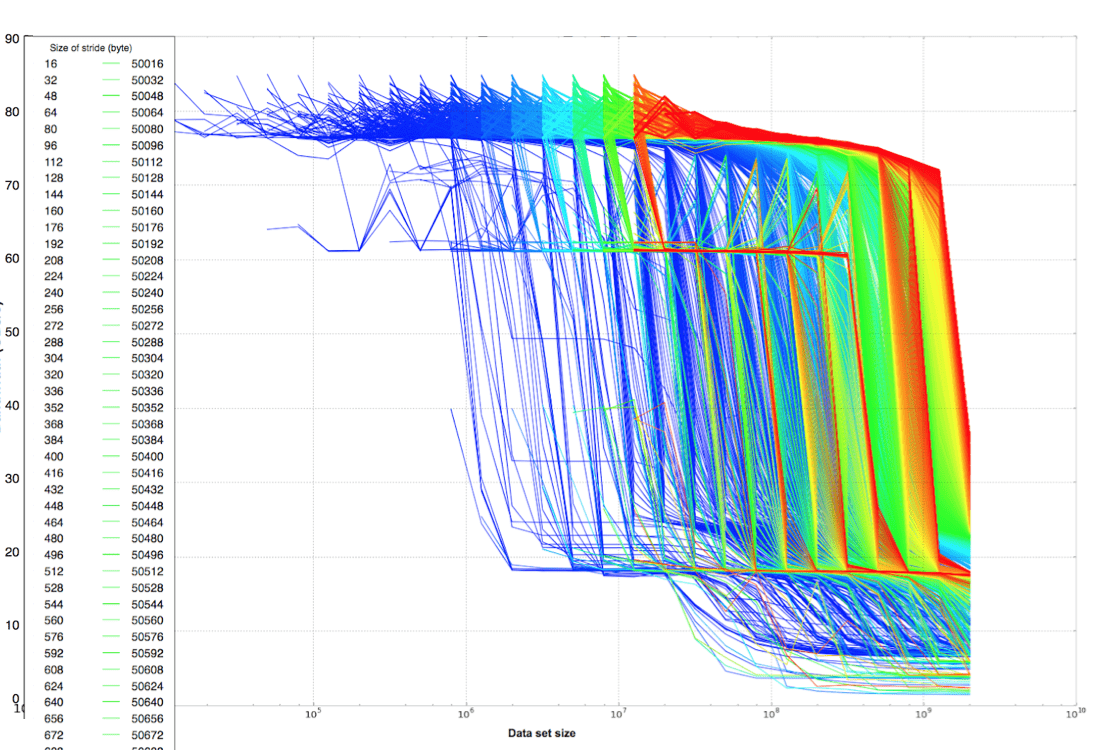
\includegraphics[width=12cm]{images/dml_strides_bad.png}
        \caption{\label{pic:dml_strides_bad} Bande passante obtenue à l'aide du benchmark \texttt{DML\_MEM} donnée en GB/s pour différentes tailles de stride représentées par des couleurs allant du bleu (petite taille) au rouge (grande taille). Nous remarquons que certaines strides de taille similaire ont des performances très inégales.}
        \end{figure}
        \textbf{TODO reprendre abscice ordonnée texte}
        
        Nous remarquons sur la \autoref{pic:dml_strides_bad} que certaines \glspl{stride} ont des comportements différents que des strides de tailles proches (donc de couleurs proches aussi). En effet, des groupes de strides ont des performances bien plus faibles que d'autres et les mêmes résultats sont obtenus en utilisant des pages larges pour réduire l'impact sur la TLB \textbf{gls}. Nous avons isolé certaines d'entre elles et reporté leur performance dans le  \autoref{tab:dml_bad_strides}. Pour réaliser ces mesures, la commande suivante a été utilisée: 
        \begin{verbatim}
./dml --steplog 0.01 --unroll 8 --mode special --type read --cacheline 64 
      --stride 73704,73728,77816,77824,81928,81920 --measure 10 --matrixsize 10000
        \end{verbatim}
        
        
        \begin{table}[ht!]
        \centering
        \begin{tabular}{|c|c|c|c|c|}
        \hline
        \rowcolor[HTML]{EFEFEF} 
        Taille de la stride (byte) & Débit mémoire mesuré (GB/s) & Nb. inst. & IPC & LLC Miss \\ \hline
        \rowcolor[HTML]{FFFFC7} 
        73704 & 24.54 & 690071400 & 0.34 & 21100474 \\ \hline
        \rowcolor[HTML]{FFFFC7} 
        73728 & 2.04 & 690064918 & 0.22 & 30612018 \\ \hline
        \rowcolor[HTML]{E8FFFE} 
        77816 & 24.53 & 688909428 & 0.33 & 21152403 \\ \hline
        \rowcolor[HTML]{E8FFFE} 
        77824 & 4.01 & 688905576 & 0.27 & 30144907 \\ \hline
        \rowcolor[HTML]{E6FFE6} 
        81928 & 24.76 & 690692156 & 0.33 & 21194483 \\ \hline
        \rowcolor[HTML]{E6FFE6} 
        81920 & 4.03 & 690693382 & 0.27 & 30794354 \\ \hline
        \end{tabular}%
        \caption{Mesure du débit mémoire atteint, du nombre d'instructions exécuté et le débit de leur exécution (Instruction Par Cycle) ainsi que le nombre de \textit{miss} mesuré dans le dernier niveau de cache (LLC) pour trois couples de strides de taille similaire.}
        \label{tab:dml_bad_strides}
        \end{table}
        
        
        Le benchmark qui utilise une \textit{mauvaise} stride (73728, 77824 ou 81920) voit sa performance limitée par la latence du système mémoire  (\textit{latency bound}). En effet, nous avons réalisé différentes mesures telles que le nombre de \textit{miss} du dernier niveau de cache ou l'activité du bus mémoire. L'analyse de l'activité du bus mémoire montre qu'il est loin d'être saturé. Si la ligne de cache n'est pas présente dans un des niveaux de cache, et que le bus n'est pas saturé, c'est que le processeur l'attend et n'a pas anticipé son manque (\textit{miss}). On remarque que l'IPC \textbf{todo gls} est plus faible et que le nombre de \textit{miss} \textbf{todo gls} est lui plus élevé pour ces strides. La question est alors de savoir pourquoi pour une certaine taille la ligne de cache est présente dans le cache et que pour une stride plus grande de quelques bytes elle n'y est pas. L'explication vient de la taille des strides utilisées. Nous avons utilisé des strides de taille $ Stride_{n+1} = Stride_n + 16 ~ bytes$ avec $Stride_0 = 16 ~ bytes$. En utilisant des tailles multiple de 16, certaines d'entre elles génèrent des conflits avec la politique de remplacement de lignes de caches. Ainsi, ces tailles de saut particulières mettent la pression seulement sur une partie du cache, le rendant inefficace. Le processeur doit donc attendre pour une majorité des accès, que la ligne de cache soit transférée depuis la mémoire. La performance du code est alors limitée par la latence du système mémoire (\textit{latency bound}).
        
        Nous avons ensuite réalisé la même expérimentation en décalant la taille des strides utilisées en commençant avec une stride minimale $Stride_0 =  8 ~ bytes$. Ainsi, aucune stride utilisée n'est multiple de 32, et aucune d'entre elles n’obtient de performance inattendue (voir \autoref{pic:dml_strides_good}).
        
        
        \begin{figure}
        \center
        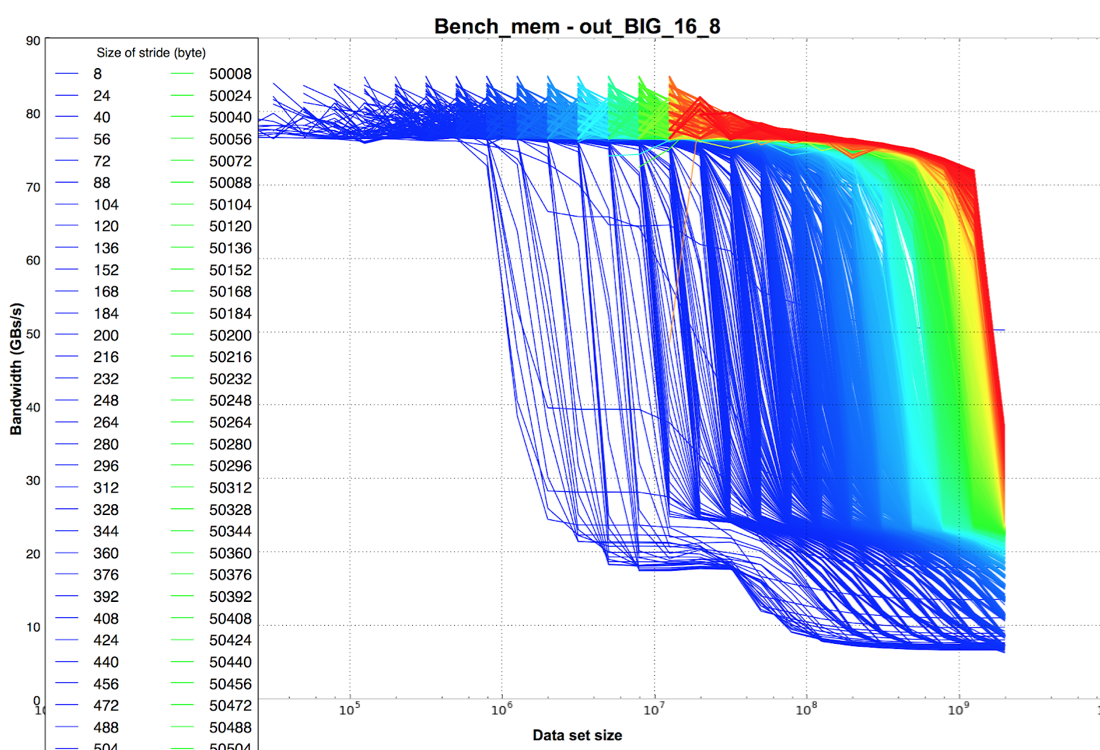
\includegraphics[width=12cm]{images/dml_strides.png}
        \caption{\label{pic:dml_strides_good} Performance du benchmark pour différentes tailles de strides (couleurs).  }
        \end{figure}
        \textbf{TODO reprendre abscice ordonnée texte + texte}
        
        À travers cette expérimentation, nous avons voulu montrer qu'un code aussi simple soit-il peut avoir des performances inattendues. La complexité des architectures modernes est telle qu'elle peut avoir une incidence forte sur la performance des applications. Pour des strides aussi longues (plusieurs MiB), le \gls{prelecteur} ne semble pas arriver à anticiper ces accès. Si une application réalise ce type d'accès, le programmeur doit s'assurer de ne pas réaliser des strides de cette taille en ajoutant du \textit{padding} (remplissage) pour décaler artificiellement les données accédées. Une autre optimisation lors d'accès à certains champs d'objets contenus dans un tableau est de regrouper ces mêmes champs dans une structure spécifique. Ainsi, ces champs sont contigus en mémoire. 
        

    \subsubsection{Saturation du bus mémoire}\label{sec:dml_saturation}
    %%%%%%%%%%%%%%%%
        Pour pouvoir modéliser la performance des applications (modèle du \textit{Roof Line}) il est courant d'utiliser les performances maximales atteignables par une ressource. Pour cela, nous avons exécuté le benchmark en utilisant différents nombres de coeurs. Les résultats sont visibles sur le graphique de la \autoref{pic:dml_bw_mpi}. Sur ce processeur, notre benchmark arrive à obtenir une bande passante mémoire maximale de 114 GB/s. À titre de comparaison, le benchmark STREAM permet d'atteindre un débit mémoire de 108 GB/s. La loi de Little ne permet pas à un seul coeur de saturer la totalité du bus mémoire. Nous montrons à travers cette expérimentation qu'il faut au moins 15 coeurs pour le saturer. Les coeurs supplémentaires ne permettent pas ensuite d'améliorer le débit mémoire, car le bus est saturé. Pour des codes \gls{memorybound}, il peut alors être intéressant d'en désactiver certains ou de ne pas investir dans des processeurs avec plus de coeurs. Nous présentons dans la \autoref{sec:dml_core_vs_freq} un script permettant de réaliser cette recherche du nombre minimal de coeurs permettant de saturer le bus mémoire. 
        
        \begin{figure}
        \center
        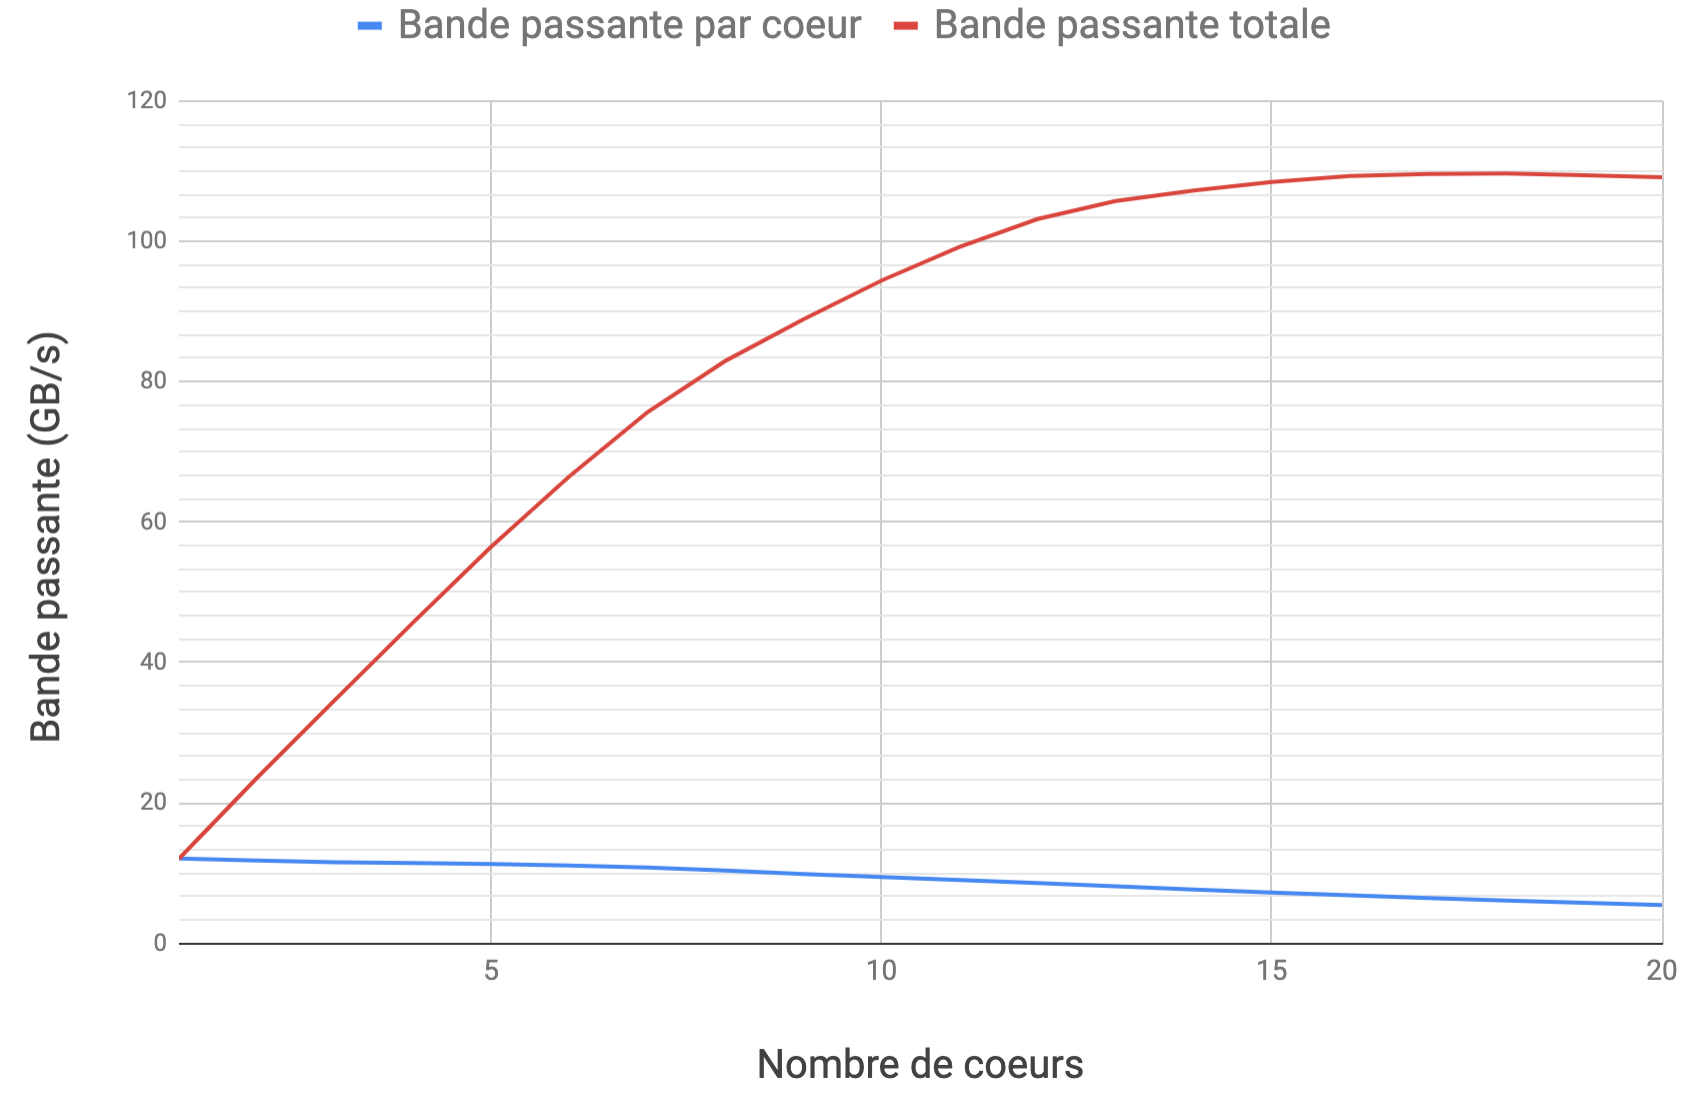
\includegraphics[width=10cm]{images/dml_bw_mpi.png}
        \caption{\label{pic:dml_bw_mpi} Bande passante mémoire atteinte pour différent nombre de coeurs}
        \end{figure}
        
    
    
    

    \subsubsection{Vérifier le bon fonctionnement des caches} \label{sec:dml_cache_ok}
    %%%%%%%%%%%%%%%%
        Les caches des architectures modernes se sont complexifiées et sont devenues très efficaces pour accélérer les accès mémoires. Cependant, sur des architectures différentes de celles utilisées communément, il peut être intéressant de vérifier leur bon fonctionnement. Nous montrons dans cette expérimentation les tests pouvant être réalisés.
        
        La première vérification est de s'assurer de l'indépendance des caches propres à chaque coeur. Dans le cas des processeurs Skylake, les deux premiers niveaux sont privés \textbf{todo privé dédié ?} à chaque coeur. Nous avons implémenté une option pour annoter la taille de niveau de cache sur le graphique final. Les résultats de deux exécutions sur 1 et 20 coeurs sont présentés sur la \autoref{pic:dml_cache}. Comme attendu, la performance du benchmark n'est pas impactée lorsque le jeu de données utilisé est situé dans les caches L1 et L2. Les performances se dégradent lorsque le jeu de données commence à remplir le dernier niveau de cache, commun à tous les coeurs.
        
        \begin{figure}
        \centering
            \begin{subfigure}[b]{0.47\linewidth}
            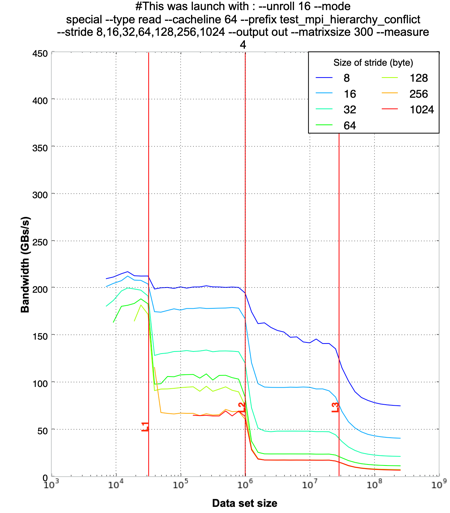
\includegraphics[width=\linewidth]{images/dml_cache_1core.png}
            \caption{Performance mesurée lors de l'utilisation d'un seul coeur}
            \label{pic:dml_cache_1core}
            \end{subfigure}
        ~ %add desired spacing between images, e. g. ~, \quad, \qquad, \hfill etc. 
        %(or a blank line to force the subfigure onto a new line)
            \begin{subfigure}[b]{0.47\linewidth}
            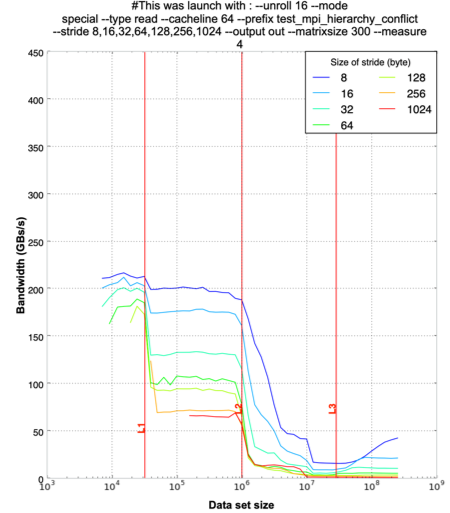
\includegraphics[width=\linewidth]{images/dml_cache_20core.png}
            \caption{Performance mesurée lorsque les vingt coeurs du processeur sont utilisés}
            \label{pic:dml_cache_20core}
            \end{subfigure}
        \caption{Performance du système mémoire mesurée à l'aide du benchmark \texttt{DML\_MEM} lors de sont exécution par 1 coeur (a) et vingt coeurs (b). Les résultats montrent que les caches L1 et L2 ne sont pas affectés par l'utilisation d'autres coeurs. Le débit mémoire disponible par coeur s'effondre lorsque plusieurs coeurs utilisent un jeu de données situé dans le cache L3.}\label{pic:dml_cache}
        \end{figure}
        
        Une deuxième expérimentation pouvant être menée au niveau des caches est la vérification du fonctionnement du cache L3. Pour cela, nous utilisons un jeu de donnée dont la taille évolue jusqu'à remplir le cache L3.  En parallèle, nous mesurons l'activité sur le bus mémoire avec l'outil \verb=YAMB=, présenté dans la \autoref{sec:yamb}. Les résultats de cette expérimentation sont montrés sur la \autoref{pic:dml_L3_sharing}. Elle a été réalisée avec les commandes suivantes:
        \begin{verbatim}
./monitoring_bw_main.sh --start
./dml --steplog 0.01 --unroll 2 --type read --cacheline 64 --stride 64  
      --matrixsize 100 --measure 1000 --minlog 6.1 --annotate log_mem.annotate
./monitoring_bw_main.sh --stop
        \end{verbatim}
        
         \begin{figure}
        \center
        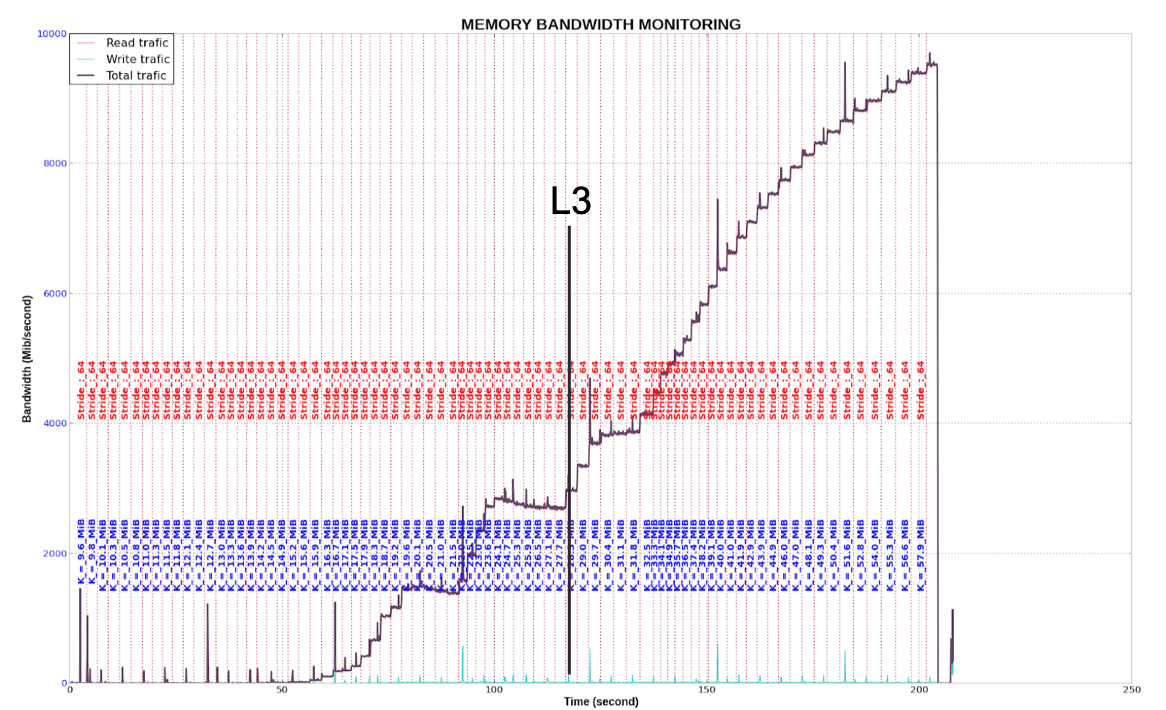
\includegraphics[width=14cm]{images/dml_L3_sharing.png}
        \caption{\label{pic:dml_L3_sharing} Évolution de l'activité du bus mémoire en fonction de la taille du jeu de donnée.}
        \end{figure}
        \textbf{TODO LARGE STP}
        
        Nous montrons ainsi qu'un cache L3 de 28 MiB ne parvient pas à garder la totalité d'un jeu de donnée dépassant les 16 MiB. Au-delà de cette taille, \verb=YAMB= mesure de l'activité sur le bus mémoire, celle-ci pouvant atteindre les 3 GB/s pour un jeu de donnée de la taille du L3 (28 MiB). Cette mauvaise utilisation du cache peut être due au phénomène de coloration de page discuté dans les expérimentations suivantes. Cette caractéristique impacte la performance de chaque coeur, car certaines données sont éjectées du cache et génèrent un évènement de \textit{miss}. Nous avons réalisé une seconde expérimentation en utilisant deux jeux de données de 20 et 28 MiB. Pour chaque jeu, nous utilisons progressivement la totalité des coeurs. Le résultat présenté sur la \autoref{pic:dml_bw_cacheL3} montre que le phénomène de \textit{trash} est encore plus fort lorsque plusieurs coeurs sont utilisés. Le trafic généré atteint les 19 GB/s pour 6 coeurs se partageant un jeu de données de 28 MiB. Cependant, la performance entre les deux benchmarks est identique, permettant de conclure au bon fonctionnement du prélecteur mémoire. Si une architecture ne possède pas un composant aussi efficace, il peut alors être intéressant de réduire la taille des jeux de données utilisés. Pour certaines optimisations comme le \textit{cache blocking}, nos expérimentations nous ont montré que le plus efficace était d'utiliser 80\% de la capacité du dernier niveau de cache.
        
        \begin{figure}
        \center
        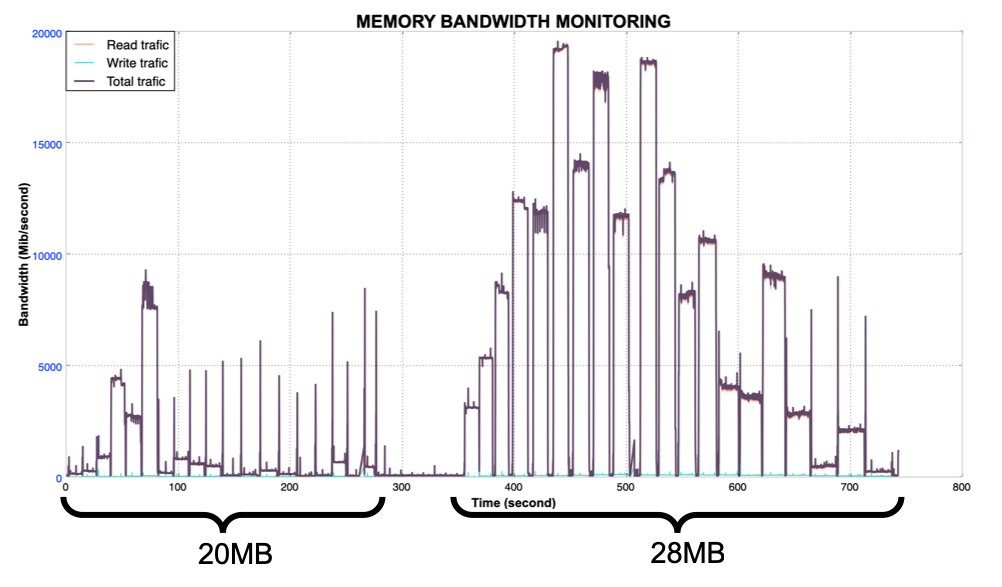
\includegraphics[width=14cm]{images/dml_bw_cacheL3.png}
        \caption{\label{pic:dml_bw_cacheL3} Évolution du trafic mémoire pour deux jeux de données de 20 et 28 MiB. Chaque jeu est accédé par 1 à 20 coeurs.}
        \end{figure}
        
        

    \subsubsection{Prélecteur mémoire}
    %%%%%%%%%%%%%%%%
        
        Dans l'expérimentation précédente, nous avons vu que le \gls{prelecteur} permettait de maintenir la bonne performance du benchmark même lorsque des données sont évincées du cache. Dans cette partie, nous questionnons l'utilité de son activation permanente à l'aide de trois expérimentations:
        \begin{enumerate}
            \item Débit mémoire atteignable par différent nombre de coeurs lors de l'activation ou non du prélecteur.
            \item Débit mémoire atteignable par un coeur lorsque le prélecteur est activé ou non pour différentes tailles de \glspl{stride}.
            \item Débit mémoire atteignable par différent nombre de coeurs lorsque le prélecteur est activé ou non pour une taille de \textit{stride} correspondant à la taille de deux lignes de cache.
        \end{enumerate}

        
       \paragraph{Impact de l'activation ou non du prélecteur.} 
            Si une architecture possède un prélecteur mémoire défaillant, il peut être intéressant de vérifier si les coeurs du processeur sont capables de générer suffisamment de requêtes mémoires pour saturer le bus.
            En utilisant la version parallèle de \verb=DML_MEM=, nous avons mesuré la performance du benchmark lorsque le mécanisme de prélecture était actif ou non, avec différent nombre de coeurs. Le benchmark a été configuré pour utiliser des sauts de 64 bytes (une ligne de cache). Ce type d'accès correspond à un algorithme de \textit{stream} accédant à toutes les données.  La \autoref{pic:dml_prefetch_mpi} montre que si le prélecteur est désactivé la totalité des coeurs ne suffisent pas à saturer le bus mémoire. Dans ce cas-là, il peut alors être intéressant de réaliser le préchargement manuellement.
        
                \begin{figure}
                \center
                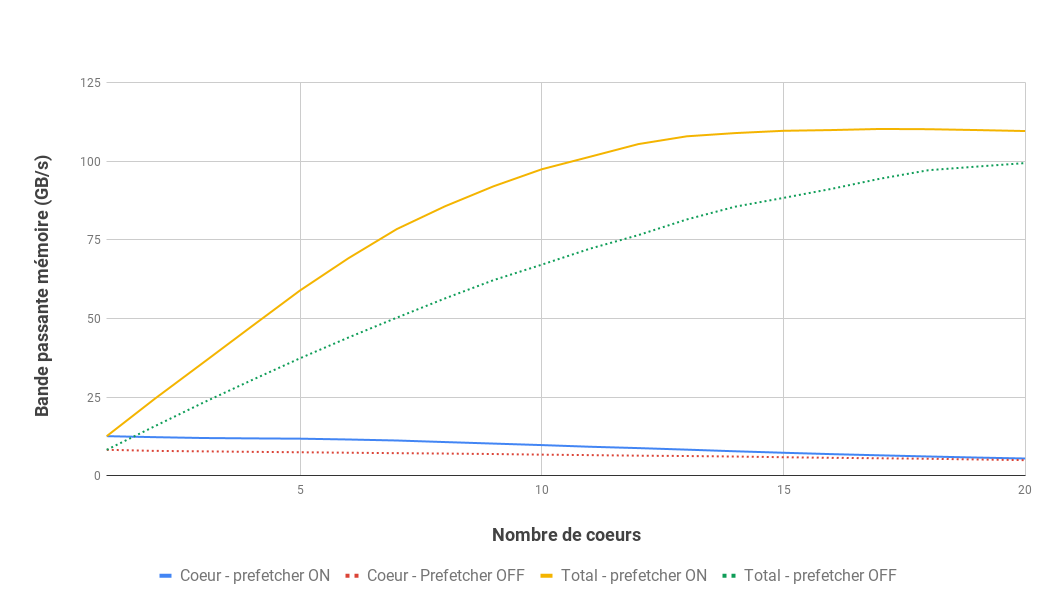
\includegraphics[width=14cm]{images/dml_prefetch_mpi.png}
                \caption{\label{pic:dml_prefetch_mpi} Performance du benchmark pour un jeu de données de 300 MiB avec un et plusieurs coeurs actifs lorsque le prélecteur adjacent est activé ou non. La stride utilisée est égale à la taille d'une ligne de cache (64 bytes).}
                \end{figure}
                \textbf{TODO plusieurs phrase + couleur + taille}

        
        \paragraph{Utilisation d'un coeur.}
            Si le prélecteur est efficace pour l'exécution d'un algorithme de \textit{stream}, il est important de vérifier son bon fonctionnement pour d'autres types d'accès. Ainsi, nous avons exécuté le benchmark \verb=DML_MEM= pour utiliser différentes tailles de \textit{strides} lors de l'accès au jeu de données lorsque le prélecteur était actif ou non. La \autoref{pic:dml_prefetch} montre le débit mémoire atteint par un seul coeur  pour des sauts allant de 64 à 3700 bytes. On remarque que les performances sont similaires sauf pour une \textit{stride} de 64 bytes, correspondant à la taille d'une ligne de cache. Pour une telle taille de \textit{stride}, la bande passante mémoire atteinte est réduite de 40\% lorsque le prélecteur est désactivé. La raison de cette baisse vient d'un mécanisme couramment utilisé dans les architectures, appelé le prélecteur adjacent (\textit{adjacent prefetch}). Les codes parcourent souvent la mémoire de façon contiguë (données d'un tableau, instruction d'un programme). Ainsi, lors d'un accès mémoire, le prélecteur adjacent anticipe les futurs accès en chargeant aussi la ligne de cache suivante. Avec l'utilisation d'une \textit{stride} de 128 bytes, nous remarquons que le mécanisme de prélecture n'améliore plus les performances, car il ne s'occupe de charger que la ligne de cache adjacente. Lorsque celui-ci est activé, le bus mémoire transfère alors des données inutilisées pouvant affecter la performance d'une application.
            
            
        
        \begin{figure}
        \center
        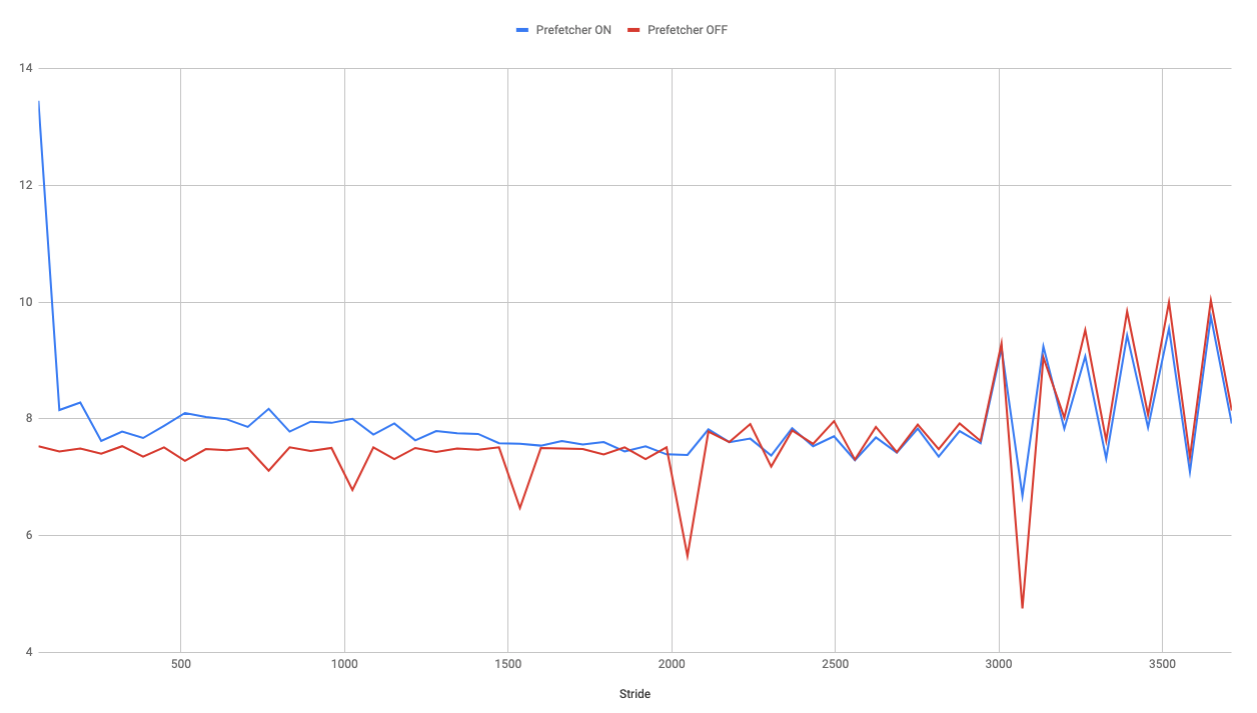
\includegraphics[width=10cm]{images/dml_prefetch.png}
        \caption{\label{pic:dml_prefetch} Débit mémoire atteint par un coeur (en GB/s) lors de l'activation (en bleu) ou non (en rouge) du prélecteur mémoire pour différentes tailles de stride. }
        \end{figure}
        
        
        
         
        \paragraph{Utilisation de tous les coeurs.} 
            
            Pour montrer que l'activation du prélecteur peut altérer les performances d'une application, la version parallèle du benchamrk \verb=DML_MEM= a été utilisée. En effet, la prélecture de la ligne de cache adjacente n'est bénéfique que si elle est ensuite utilisée. Lorsqu'un seul coeur est actif, le chargement de cette ligne de cache n'impacte pas la performance du benchmark, car le bus est loin d'être saturé. En effet, un seul coeur n'est pas capable de générer un trafic supérieur à 10 GB/s alors que le bus mémoire peut assurer un débit dépassant 110 GB/s (voir \autoref{pic:dml_prefetch}). 
            
            Afin de montrer l'impact que pourrait avoir l'activation du prélecteur mémoire, nous avons utilisé la version parallèle de \verb=DML_MEM= pour charger la totalité des coeurs du processeur. Le benchmark a alors été utilisé pour réaliser un accès mémoire avec un saut de 128 bytes correspondant à deux lignes de cache. Ainsi, nous avons pu mesurer l'impact du prélecteur mémoire qui utilise le bus mémoire pour transférer 50\% de données inutiles. Ainsi, les performances atteintes lorsque le prélecteur est désactivé sont augmentée de 16\% (91 GB/s contre 73 GB/s) \textbf{todo revoir ça}. Ce type d'accès \textbf{todo de quoi ?}, plus grand que deux lignes de cache, est très courant dans les applications. Il peut donc être avantageux de désactiver le prélecteur de la ligne de cache adjacente pour ces portions de codes. De plus, le prélecteur de données peut être réalisé manuellement grâce à des instructions telles que \verb| __builtin_prefetch (&a[i+j]); |.





    
    \subsubsection{Déroulement de boucle} \label{sec:dml_unroll}
    %%%%%%%%%%%%%%%%
    Pour améliorer les performances du benchmark \verb=DML_MEM=, l'optimisation du déroulement de boucle a été utilisée. Au vu de l'amélioration des performances obtenues, cette section présente comment l'optimisation est implémentée et comment les applications peuvent en tirer partie. 
    Le déroulement de boucle est une optimisation permettant de réduire l'impact du code responsable du contrôle de la boucle (le test de continuité et l'incrémentation). Le principe est de dérouler manuellement le code de plusieurs itérations dans la boucle et d'incrémenter le compteur du même nombre de déroulements. Ainsi, la proportion de code responsable du contrôle de la boucle est réduite par rapport à l'intérieur de la boucle. 
    
    \paragraph{Première implémentation.}
    
        Une première version du code utilisé pour réaliser le déroulement est présentée dans l'\autoref{lst:dml_unroll_orig}. Pour permettre au processeur commencer les accès mémoire grâce au mécanisme d'exécution dans le désordre, 4 pointeurs différents sont utilisés. Chaque pointeur pointe vers une stride et la valeur est sommée dans la variable \verb|sum|.  
    
        \begin{lstlisting}[label=lst:dml_unroll_orig ,language=C, caption=Première version du déroulement de la boucle par 4.]
for (rep = 0; rep < repeat; rep++) {
    DML_DATA_TYPE *p1 = mat;
    DML_DATA_TYPE *p2 = p1 + step;
    DML_DATA_TYPE *p3 = p2 + step;
    DML_DATA_TYPE *p4 = p3 + step;
    for (steps = 0; steps < ops_per_scan; steps++) {
        sum += *p1;
        p1 += xstep;
        sum += *p2;
        p2 += xstep;
        sum += *p3;
        p3 += xstep;
        sum += *p4;
        p4 += xstep;
    }
}
\end{lstlisting}
    
         Les résultats obtenus par cette première version sont mauvais, notamment pour des jeux de données situés dans les premiers niveaux de cache (baisse de la performance d'un facteur trois). Cet effondrement de performance vient de l'incapacité du compilateur à appliquer sa propre optimisation de déroulement de boucle. Cette première version étant plus mauvaise, la performance est fortement dégradée. Par ce premier résultat, nous souhaitons attirer l'attention du programmeur sur le fait que le compilateur réalise déjà certaines optimisations. Il peut être contre-productif de les réaliser soi-même.

    \paragraph{Deuxième implémentation.}
    
        L'erreur dans la première version du déroulement est l'utilisation d'une unique variable de sommation (\verb=sum=). En effet, cette variable doit être incrémentée à chaque lecture d'une stride et crée une dépendance en écriture, empêchant le code d'exécuter deux opérations d'addition par cycle. L'\autoref{lst:dml_unroll_spe} présente la version \textit{special} de l'optimisation du déroulement qui utilise autant de variables de sommation que de déroulements réalisés. Avec cette version, la performance du benchmark dans les caches L1 et L2 est améliorée respectivement de 12\% et 30\% par rapport à la version non-optimisée (produite par le compilateur).
    
    \begin{lstlisting}[label=lst:dml_unroll_spe ,language=C, caption=Deuxième version du déroulement par 4 utilisant 4 variables sum.]
for (rep = 0; rep < repeat; rep++) {
    BM_DATA_TYPE *p1 = mat;
    BM_DATA_TYPE *p2 = p1 + step;
    BM_DATA_TYPE *p3 = p2 + step;
    BM_DATA_TYPE *p4 = p3 + step;
    for (steps = 0; steps < ops_per_scan; steps++) {
        sum1 += *p1;
        p1 += xstep;
        sum2 += *p2;
        p2 += xstep;
        sum3 += *p3;
        p3 += xstep;
        sum4 += *p4;
        p4 += xstep;
    }
}
return sum1 + sum2 + sum3 + sum4;
\end{lstlisting}
    
    \paragraph{Recherche du nombre optimal de déroulements de la boucle.}
    
        La suite de cette expérimentation s'intéresse au nombre de déroulements de la boucle et de son impact sur la performance du benchmark. Pour cela, le benchmark a été exécuté en utilisant entre 1 et 64 déroulements sur un jeu de données remplissant 80\% du cache de niveau 2. Les résultats obtenus sont présentés dans le \autoref{tab:dml_unroll_bench}. Nous vérifions que l'optimisation du déroulement est bénéfique pour la performance du benchmark, ce qui améliore les performances progressivement de 117.8 GB/s à 337 GB/s pour un déroulement de boucle allant de 2 à 8 fois. On remarque que moins d'instructions sont exécutées et que le nombre d'instructions exécutées chaque cycle augmente de 2 à 3.22. Au-delà de 8 déroulements, la performance du benchmark se dégrade progressivement. Avec 64 déroulements de la boucle, le nombre d'instructions exécutées double et les performances s'effondrent à 140 GB/s. Cette expérimentation nous permet de montrer que la mesure du nombre d'instructions exécutées chaque cycle (IPC) \textbf{todo glossaire} n'est pas un indicateur suffisant pour évaluer la performance d'un code. 
    
    
        \begin{table}[ht!]
        \centering
        \begin{tabular}{|c|c|c|c|}
        \hline
        \rowcolor[HTML]{EFEFEF} 
        \multicolumn{1}{|l|}{\cellcolor[HTML]{EFEFEF}Nb. de déroulements} & \multicolumn{1}{l|}{\cellcolor[HTML]{EFEFEF}Bande passante (GB/s)} & \multicolumn{1}{l|}{\cellcolor[HTML]{EFEFEF}Nb. d'instructions exécutée}s & \multicolumn{1}{l|}{\cellcolor[HTML]{EFEFEF}Instruction par cycle} \\ \hline
        1 & 117.8 & 4204612342 & 2 \\ \hline
        2 & 235.47 & 3159994082 & 2.99 \\ \hline
        4 & 311.07 & 2634059908 & 3.28 \\ \hline
        8 & 337.96 & 2380891060 & 3.22 \\ \hline
        16 & 306.66 & 2483260088 & 3.07 \\ \hline
        32 & 315.17 & 2513084995 & 3.19 \\ \hline
        64 & 140.98 & 4993000253 & 2.87 \\ \hline
        \end{tabular}%
        \caption{Performance du benchmark \texttt{DML\_MEM} utilisant plusieurs tailles de déroulement de la boucle pour un jeu de donnée atteignant 80\% du cache L2 pour une stride de 64 byte.}
        \label{tab:dml_unroll_bench}
        \end{table} \textbf{todo ca dépasse}
        
        Pour comprendre la mauvaise performance du code lorsqu'il est déroulé plus de 8 fois, nous avons extrait leur code assembleur. L'\autoref{lst:unroll4} montre comment le code du benchmark est généré lorsque 4 déroulements sont réalisés. On remarque que les 4 opérations d'addition sont vectorisées et qu'elles se suivent dans le code, permettant au mécanisme d'exécution dans le désordre, de les exécuter deux par deux. On remarque aussi que 16 des 32 registres \verb|%xmm| sont utilisés. L'\autoref{lst:unroll16} expose le code assembleur du benchmark déroulant 16 fois la boucle. Le processeur utilise alors la totalité des 32 registres \verb|%xmm|. Cependant, ce n'est pas suffisant pour réaliser tous les traitements et il est obligé de stocker et charger certains éléments depuis la pile. L'exécution des opérations d'addition vectorisées est alors ralentie. Pour comprendre l'effondrement des performances lors de 64 déroulements, l'analyse du code assembleur est une fois de plus précieuse. Lorsque 64 déroulements sont utilisés, le compilateur ne parvient plus à générer d'additions vectorielles. Les performances sont alors divisées par deux, alors que l'IPC est presque similaire. 
        

\begin{minipage}{.45\textwidth}
\begin{lstlisting}[
label=lst:unroll4,
basicstyle={\scriptsize\ttfamily},
identifierstyle={\color{black}},
language={[x86masm]Assembler},
tabsize=2,
numbersep=8pt,
frame=tlbr,framesep=2pt,framerule=0pt,
morekeywords ={class,run},
caption=Boucle déroulée 4 fois.
]
vmovhpd (%r14,%r11,8),%xmm8,%xmm9
lea     (%rsi,%r12,8),%r14
vmovhpd (%r15,%r11,8),%xmm10,%xmm11
lea     (%r12,%r11,2),%r12
vmovsd  (%r15),%xmm14
vmovhpd (%r14,%r11,8),%xmm12,%xmm13
vmovhpd (%r15,%r11,8),%xmm14,%xmm15
vaddpd  %xmm9,%xmm3,%xmm3
vaddpd  %xmm11,%xmm2,%xmm2
vaddpd  %xmm13,%xmm1,%xmm1
vaddpd  %xmm15,%xmm0,%xmm0
\end{lstlisting}
\end{minipage}%%
\hfill
%&
%
\begin{minipage}{.45\textwidth}
\begin{lstlisting}[
label=lst:unroll16,
basicstyle={\scriptsize\ttfamily},
identifierstyle={\color{black}},
tabsize=2,
language={[x86masm]Assembler},
numbersep=8pt,
xleftmargin=0.5cm,frame=tlbr,framesep=2pt,framerule=0pt,
morekeywords ={class,run},
caption=Boucle déroulée 16 fois.
]
vmovsd  (%r15),%xmm30
vmovhpd (%r15,%r9,8),%xmm30,%xmm30
lea     (%r14,%rdx,8),%r15
vaddpd  %xmm30,%xmm31,%xmm31
vmovsd  (%r15),%xmm30
vmovhpd (%r15,%r9,8),%xmm30,%xmm30
lea     (%r11,%rdx,8),%r15
vaddpd  %xmm30,%xmm3,%xmm3
. 
. 
. 
\end{lstlisting}
\end{minipage}
    
        
        Pour mieux apprécier les performances de chaque déroulement, le benchmark est exécuté dans les différents niveaux de la hiérarchie mémoire. Les résultats sont présentés sur le graphique de la \autoref{pic:dml_unroll_best}. Dans le cache L1, l'utilisation de 4 et 8 pointeurs permet d'améliorer la performance de 40 GB/s. On remarquera aussi la mauvaise performance de deux déroulements de la boucle dans ces premiers niveaux de caches. Cette expérimentation permet de montrer que la manière optimale d'accéder à un jeu de données présent dans les caches est d'utiliser entre 4 et 8 pointeurs différents. Au-delà, le nombre restreint de registres disponibles pour le processeur détériore la performance. La performance dans les caches des versions avec 4, 8 ou 16 déroulements est supérieure à celle du compilateur \verb|ICC| (correspondant à un déroulement de 1 dans la \autoref{pic:dml_unroll_best}). Lorsque les données sont dans la mémoire, le déroulement n'améliore pas les performances (voire les dégrade). 
    
        \begin{figure}
        \center
        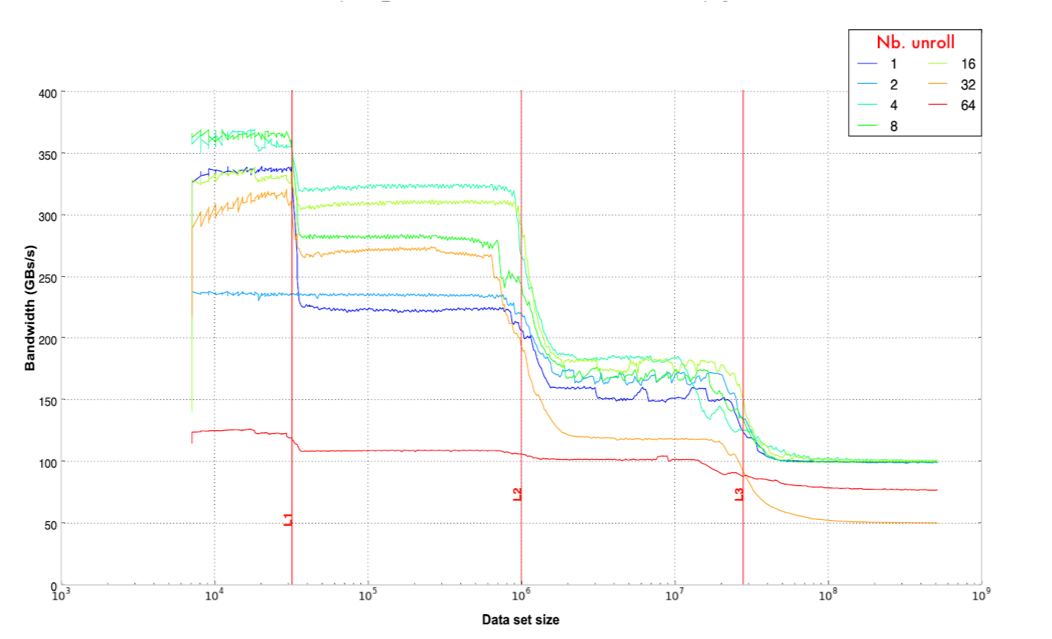
\includegraphics[width=16cm]{images/dml_unroll_best.png}
        \caption{\label{pic:dml_unroll_best} Performance de plusieurs déroulements pour une stride de 8 bytes (lecture de tous les éléments).}
        \end{figure}
        \textbf{TODO PLUS GROS}
    
    \subsubsection{Large page} \label{sec:dml_large_page}
    %%%%%%%%%%%%%%%%

    L'expérimentation suivante a pour objectif de comparer la performance du benchmark lors de l'utilisation de différentes tailles de pages mémoire. Comme présenté dans l'\aref{sec:page}, l'utilisation de page de plus grande taille permet d'améliorer la performance du système mémoire, notamment en accélérant le traitement de la TLB \textbf{todo gls}. Les pages plus larges permettent aussi de réduire les conflits d'associativité dans les caches. L'expérimentation réalisée avec un coeur actif a permis d'obtenir les résultats présentés dans le \autoref{tab:large_page_memory}. La performance des caches est améliorée avec l'utilisation des pages larges, jusqu'à 30\% dans le cache L3. Lorsque le jeu de données est dans le cache de niveau 3, la mesure du nombre d'évènements \textit{miss} de la TLB augmente d'un facteur 300. Cependant, la TLB arrive à masquer la majorité de ces \textit{miss} et conserve une bonne performance (150 GB/s).

    \begin{table}
    \centering
    %\resizebox{\textwidth}{!}{%
    \begin{tabular}{l|c|c|c|c|c|}
    \cline{2-6}
     & \cellcolor[HTML]{EFEFEF}L1 (GB/s) & \cellcolor[HTML]{EFEFEF}L2 (GB/s) & \cellcolor[HTML]{EFEFEF}L3 (GB/s) & \cellcolor[HTML]{EFEFEF}Memoire (GB/s) & \cellcolor[HTML]{EFEFEF}dTLB-load-misses \\ \hline
    \multicolumn{1}{|l|}{\cellcolor[HTML]{EFEFEF}Page de 4 KiB} & 320 & 220 & 150 & 13.40 & 2254025 \\ \hline
    \multicolumn{1}{|l|}{\cellcolor[HTML]{EFEFEF}Page de 2 MiB} & 340 & 225 & 200 & 13.45 & 6556 \\ \hline
    \end{tabular}%
    %}
    \caption{Performance du benchmark \texttt{DML\_MEM} utilisant deux tailles de pages. Le débit des 4 niveaux de la hiérarchie mémoire (GB/s) a été mesurée en utilisant une stride de 64 bytes. Le nombre d'évènements \textit{miss} correspond à l'exécution du benchmark avec un jeu de donnée situé dans le cache L3.}
    \label{tab:large_page_memory}
    \end{table}
    
    
    Nous nous sommes ensuite intéressés aux performances du benchmark lorsque plusieurs coeurs sont actifs, avec et sans l'utilisation des pages larges. Nous observons les mêmes écarts de performances lorsque le jeu de données est stocké dans les caches. Lors de l'utilisation de pages standards (4 KiB), nous constatons que lorsque la taille du jeu de données approche de la taille d'un niveau de cache, la performance commence à se détériorer. Avec l'utilisation des pages de 4 MiB, la performance dans chaque niveau de cache est constante et ne se détériore que lorsque le jeu de donnée dépasse la taille du niveau de cache. Cet effet observé lors de l'utilisation de petites pages est appelé \textit{page coloring}\footnote{La coloration de page est une technique logicielle permettant d'améliorer le mappage d'une page de la mémoire physique sur les lignes de cache du processeur. Cette technique permet d'assurer que des pages contiguës en mémoire virtuelle sont allouées à des pages physiques qui se répartiront efficacement dans les caches.} \cite{Zhang2009}.
  
    \begin{figure}
    \center
    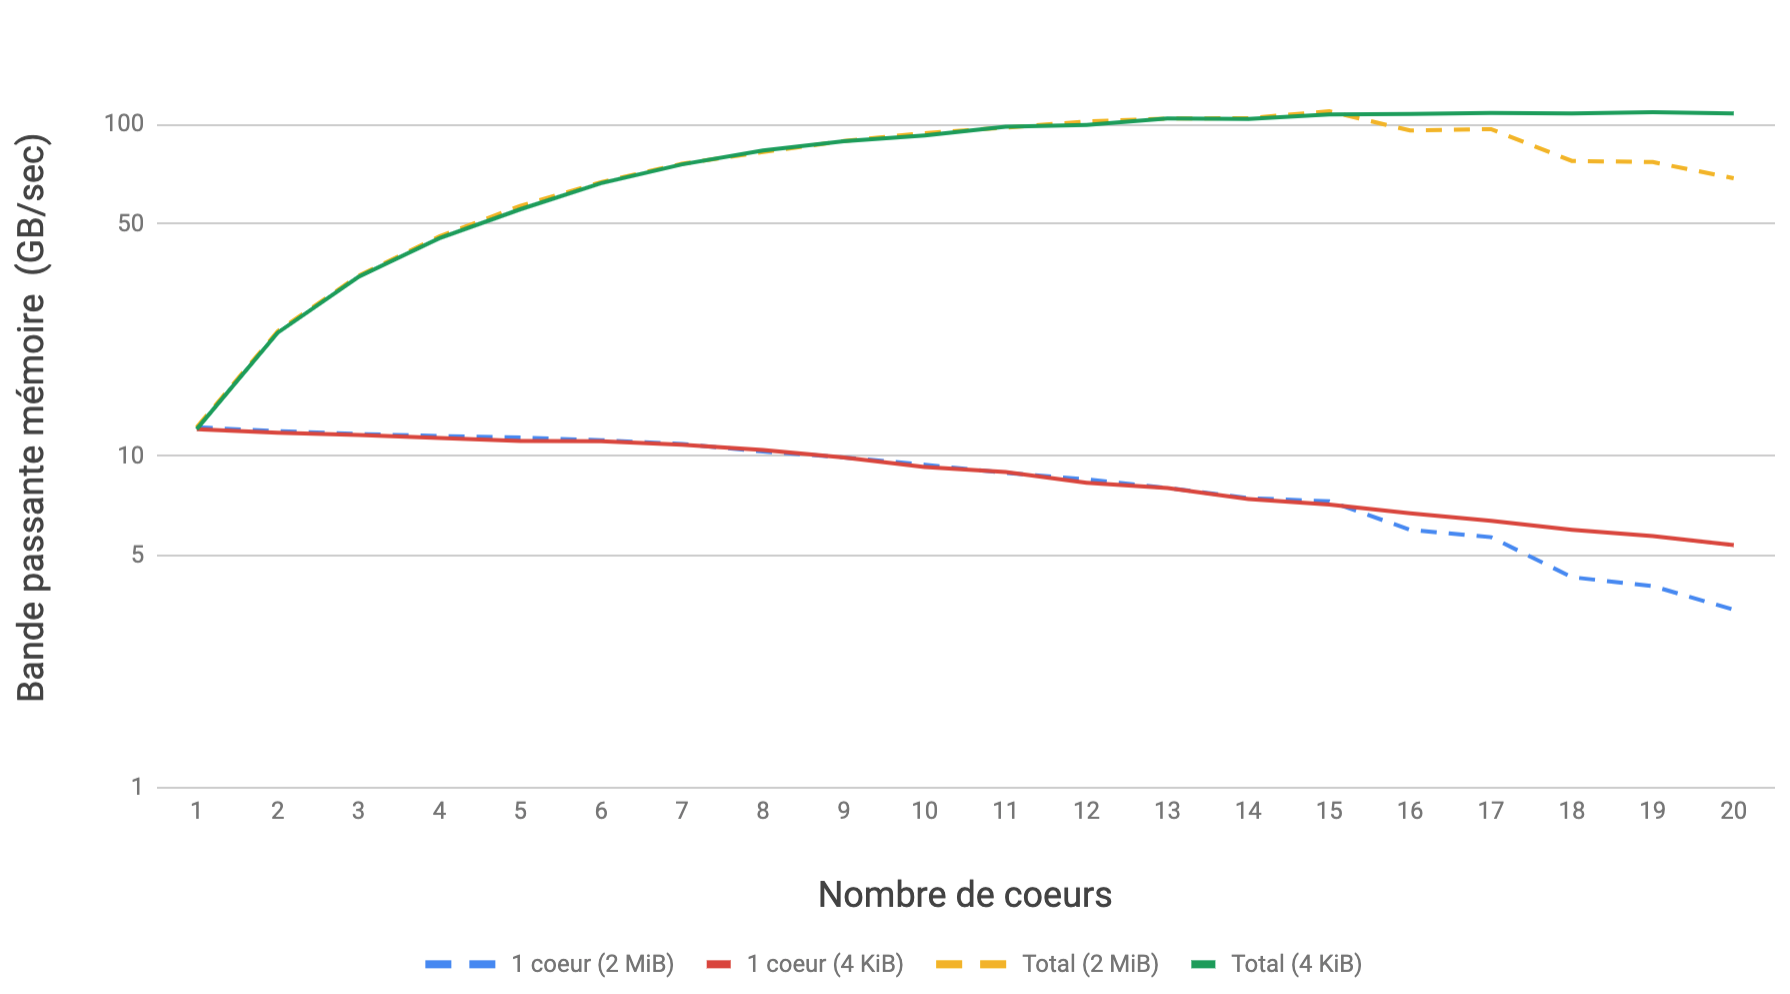
\includegraphics[width=14cm]{images/dml_large_page_bw.png}
    \caption{\label{pic:dml_large_page_bw} Débit mémoire mesuré en GB/s atteint par un coeur (rouge et bleu) et par différents nombre de coeurs (jaune et vert) utilisant des pages de 4 KiB (rouge et vert) et 2 MiB (bleu et jaune) pour accéder à un jeu de données de 2 GiB.}
    \end{figure}
    
    Le graphique de la \autoref{pic:dml_large_page_bw} montre les performances du benchmark avec un ou plusieurs coeurs actifs sur un jeu de donnée de 2 GiB. Nous remarquons que la performance du benchmark baisse lorsque plus de 15 coeurs sont utilisés avec des pages larges. La performance par coeur diminue de 5.39 GB/s à 3.44 GB/s alors que le bus mémoire n'est pas saturé. Nous n'avons pour le moment pas réussi à expliquer ce problème qui affecte tous les jeux de données supérieurs à 2 GiB.
    
    Bien que la TLB limite rarement les performances des applications réelles, le recours à l'utilisation de pages larges peut être bénéfique. Les versions récentes du noyau Linux peuvent choisir elles-mêmes lors de l'allocation mémoire si le recours à des pages plus grandes peut être bénéfique pour l'application (Red Hat Transparent Huge Pages (THP)). Comme nous montrons dans cette dernière expérience que l'utilisation de pages de 2 MiB peut détériorer les performances, nous préconisons que ce choix revienne à l'utilisateur. Il devra décider ou non de leur utilisation, en fonction de application utilisée. 
  


    
    \subsubsection{Fréquence et coeurs: impact sur le débit mémoire} \label{sec:dml_core_vs_freq}
    %%%%%%%%%%%%%%%%
    
    Dans cette expérimentation nous avons mesuré la bande passante mémoire atteignable par notre benchmark pour différente configuration de fréquence et nombre de coeurs actifs. Les résultats sont visibles sur la \autoref{pic:dml_core_vs_freq}. Comme dans l'expérimentation précédente (\autoref{sec:dml_saturation}), nous démontrons que la totalité des coeurs n'est pas nécessaire pour saturer la bande passante. Cette expérience montre aussi que les coeurs utilisés n'ont pas besoin d'utiliser leur fréquence maximale. En effet, notre benchmark sature le bus mémoire avec 17 coeurs cadencés à seulement 2.1 GHz. Le script utilisé pour générer la \autoref{pic:dml_core_vs_freq} annote automatiquement le graphique pour identifier rapidement les maximums. Une telle utilisation du benchmark \verb=DML_MEM= permet d'identifier le couple  \verb|{fréquence, nombre de coeurs}| minimal pour saturer le bus mémoire. Pour des applications limitées par la performance de ce dernier, il peut être intéressant de désactiver les coeurs supplémentaires ou de plafonner la fréquence du processeur pour limiter la consommation électrique. En plus de vérifier la présence potentielle de bogues dans l'architecture, cette expérimentation peut permettre à un utilisateur de choisir la meilleure configuration pour un achat de nouveaux processeurs. 
    
    \begin{figure}[ht]
    \center
    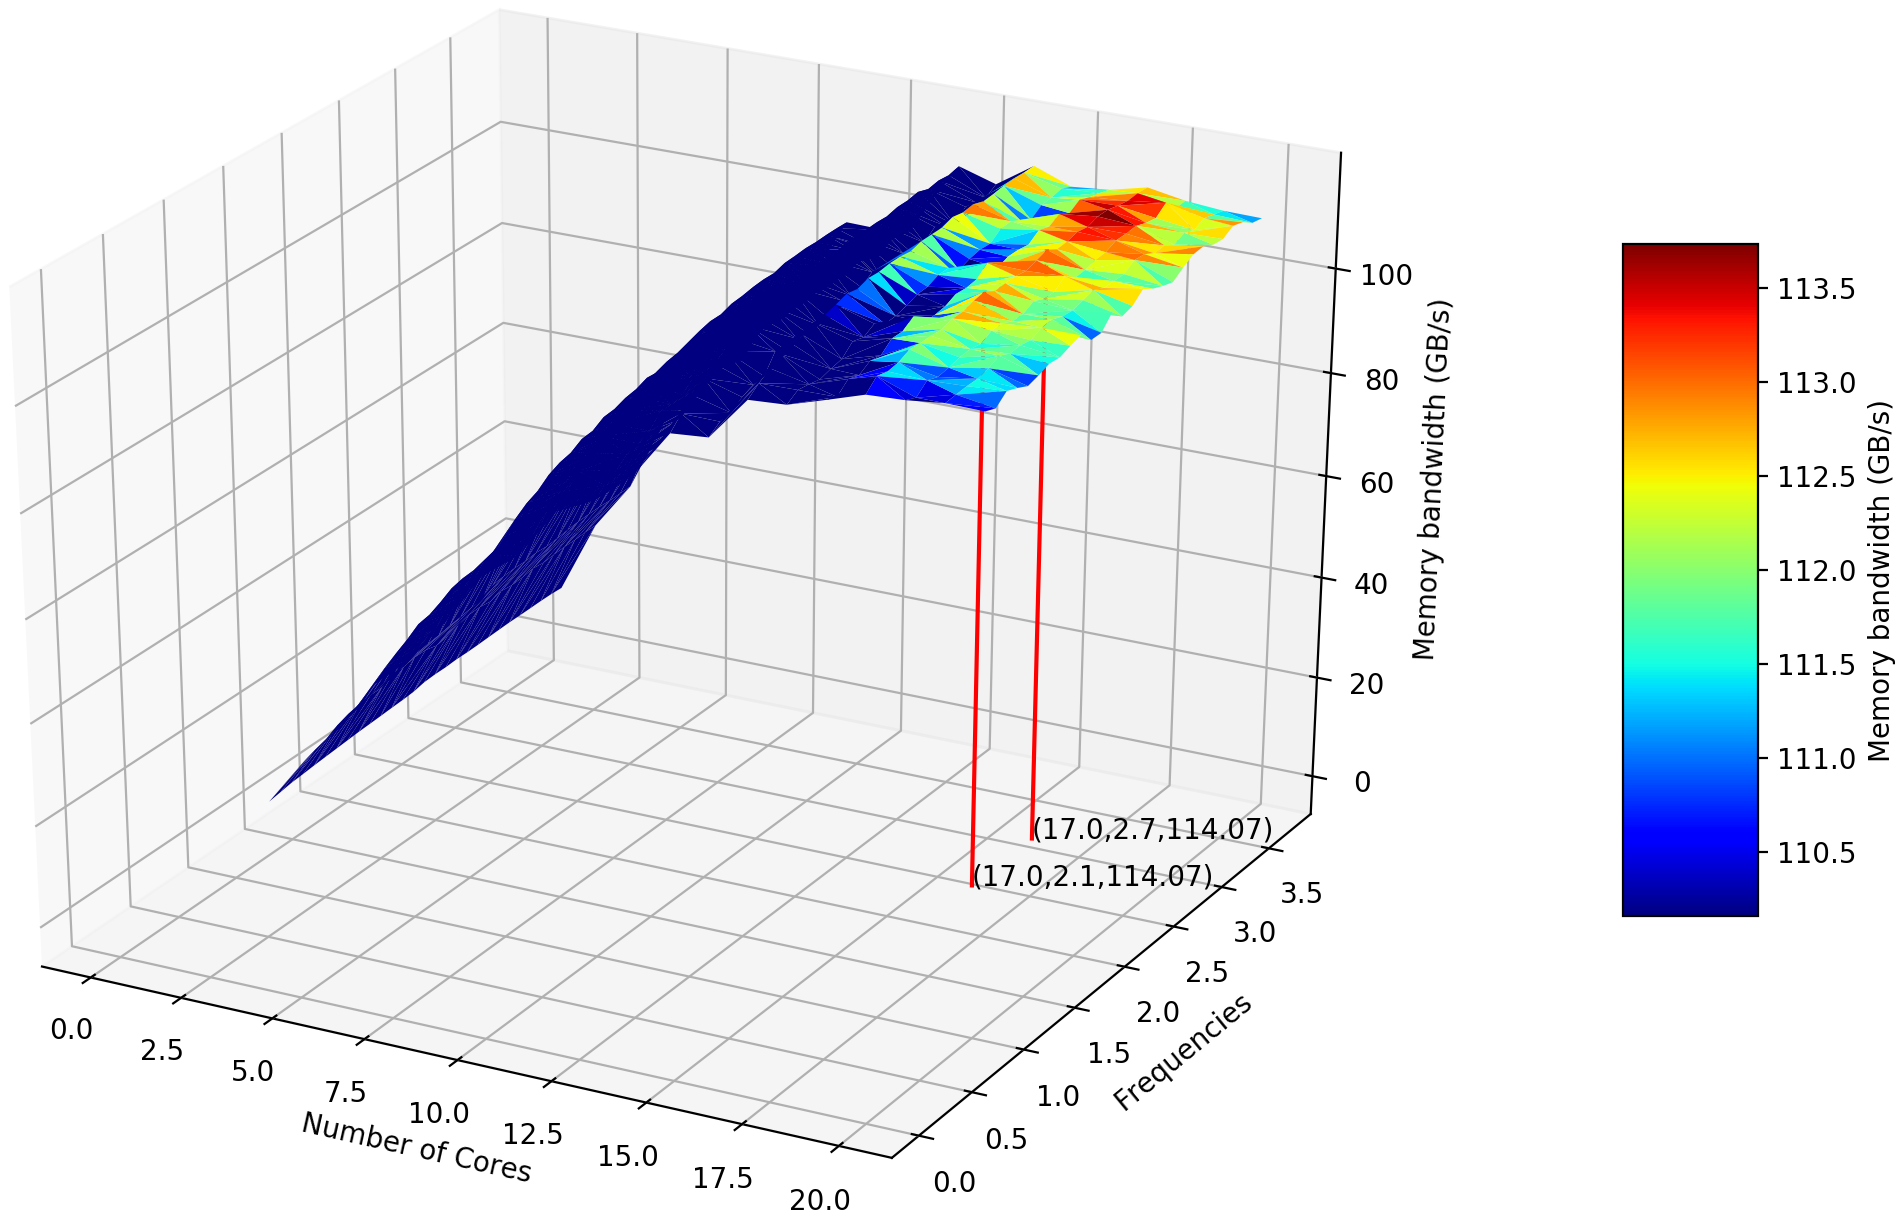
\includegraphics[width=14cm]{images/dml_core_vs_freq.png}
    \caption{\label{pic:dml_core_vs_freq}  Mesure du débit du bus mémoire (en GB/s) atteint par le benchmark lors de l'utilisation de différents nombres de coeurs dont la fréquence est comprise entre XX et XX \textbf{TODO} (en GHz). Le débit maximal atteint pour ce processeur est de 114.07 GB/s en utilisant 17 coeurs cadencés à 2,1 ou 2,7 GHz.}
    \end{figure}
    


    
    

\subsection{Conclusion}
%%%%%%%%%%%%%%%%%%%%%%%%%%%%%%%%%%%%%%%%%%%%%%%%%%%%%%

    Cette section s'intéresse au benchmark \verb=DML_MEM=, un outil permettant de caractériser de multiples parties du système mémoire. Le benchmark utilise des accès mémoire par saut, appelés \glspl{stride} et nous a permis de caractériser plusieurs parties de la microarchitecture. Une première utilisation nous a permis de déduire la taille d'une ligne de cache, donnée importante pour la programmation efficace d'applications. En utilisant différentes tailles de strides, nous avons pu mesurer l'impact que celles-ci pouvaient avoir sur la performance des différents niveaux de la hiérarchie mémoire. En utilisant une taille de stride correspondant à la taille d'une ligne de cache, nous avons pu caractériser l'architecture pour l'exécution d'algorithmes de streaming. Nous avons ainsi pu mesurer le débit maximal atteignable par le bus mémoire. Lors de nos expérimentations, nous avons obtenu des débits supérieurs (de l'ordre de 5\%) à ceux obtenus grâce au benchmark \verb|STREAM| \cite{McCalpin1995}. Nous avons ensuite utilisé le benchmark \verb=DML_MEM= pour exposer la complexité des microarchitectures modernes. Nous montrons que la microarchitecture peut avoir des comportements inattendus lors de l'utilisation de certaines tailles de saut. À travers ces expérimentations, nous souhaitons attirer l'attention du programmeur sur la complexité de la microarchitecture et de la nécessité de sa caractérisation. Nous avons pu voir que les performances atteintes par un code aussi simple pouvaient varier de plusieurs ordres de grandeur à cause de paramètres subtils: préchargement mémoire, taille des pages, nombre de déroulements de boucle...
    
    
    Lors des travaux de thèse, l'utilisation de cet outil nous a permis de caractériser plusieurs plateformes différentes et de déceler un bogue majeur dans un nouvel accélérateur. Ce bogue, inconnu par l'entreprise l'ayant conçue, condamne les applications utilisant des motifs de calculs de type Stencil, à n'accéder qu'à une fraction des performances mémoires théoriques de l'accélérateur. Ce travail réalisé pour un client industriel ne peut cependant pas être rendu public dans ce manuscrit.